\documentclass[11pt,a4paper]{article}
\usepackage[margin=2.5cm]{geometry}
\usepackage[T1]{fontenc}
\usepackage[utf8]{inputenc}
\usepackage[expansion=false]{microtype}

\usepackage{amsmath,amssymb,amsthm}
\usepackage{booktabs,graphicx,float,caption}
\usepackage[colorlinks=true,linkcolor=black,citecolor=black,urlcolor=blue]{hyperref}
\usepackage[numbers,sort&compress]{natbib}
\usepackage{xcolor}
\captionsetup{font=small,labelfont=bf}
\newtheorem{proposition}{Proposition}
\newtheorem{lemma}{Lemma}
\newcommand{\todo}[1]{\textcolor{red}{[TODO: #1]}}
\newcommand{\pending}[1]{\textcolor{red}{[PENDING: #1]}}
\newcommand{\Hone}{H_{1}}
\newcommand{\Hzero}{H_{0}}
\newcommand{\Fii}{\mathbb{F}_{2}}
\newcommand{\Bflip}{B}
\newcommand{\dchange}{\delta}
\newcommand{\Lup}{L^{\uparrow}}
\newcommand{\Ldown}{L^{\downarrow}}
\newcommand{\R}{\mathbb{R}}
\newcommand{\supp}{\operatorname{supp}}
\newcommand{\rank}{\operatorname{rank}}
\newcommand{\pers}{\operatorname{pers}}

% Code repository and the commit that holds every result file used here.
\newcommand{\coderepo}{\url{https://github.com/DrJeni-TDA/brca-tda}}
\newcommand{\resultscommit}{\texttt{11b32a7}}

% Generated by brca-tda/scripts/paper_numbers.py. Do not edit by hand.
\newcommand{\calNormalN}{1,000}
\newcommand{\calNormalL}{4.9}
\newcommand{\calNormalLci}{3.6--6.4}
\newcommand{\calNormalG}{5.6}
\newcommand{\calNormalGci}{4.3--7.2}
\newcommand{\calNormalKS}{0.90}
\newcommand{\calTthreeN}{500}
\newcommand{\calTthreeL}{6.0}
\newcommand{\calTthreeLci}{4.1--8.5}
\newcommand{\calTthreeG}{4.0}
\newcommand{\calTthreeGci}{2.5--6.1}
\newcommand{\calTthreeKS}{0.04}
\newcommand{\calSkewedN}{500}
\newcommand{\calSkewedL}{5.2}
\newcommand{\calSkewedLci}{3.4--7.5}
\newcommand{\calSkewedG}{3.4}
\newcommand{\calSkewedGci}{2.0--5.4}
\newcommand{\calSkewedKS}{0.97}
\newcommand{\decOneN}{200}
\newcommand{\decOneChanged}{15}
\newcommand{\decTwoN}{200}
\newcommand{\decTwoChanged}{15}
\newcommand{\pairAOne}{61}
\newcommand{\pairAOneci}{54--68}
\newcommand{\aucAOne}{0.51}
\newcommand{\tcycAOne}{-3.10}
\newcommand{\tmodAOne}{-3.19}
\newcommand{\pairATwo}{72}
\newcommand{\pairATwoci}{65--78}
\newcommand{\aucATwo}{0.52}
\newcommand{\tcycATwo}{-6.05}
\newcommand{\tmodATwo}{-6.53}
\newcommand{\pairArankOne}{60}
\newcommand{\pairArankOneci}{52--66}
\newcommand{\aucArankOne}{0.50}
\newcommand{\tcycArankOne}{-2.27}
\newcommand{\tmodArankOne}{-2.37}
\newcommand{\pairArankTwo}{75}
\newcommand{\pairArankTwoci}{68--81}
\newcommand{\aucArankTwo}{0.53}
\newcommand{\tcycArankTwo}{-4.21}
\newcommand{\tmodArankTwo}{-4.88}
\newcommand{\pairZOne}{70}
\newcommand{\pairZOneci}{63--76}
\newcommand{\aucZOne}{0.52}
\newcommand{\tcycZOne}{-2.24}
\newcommand{\tmodZOne}{-2.49}
\newcommand{\pairZTwo}{80}
\newcommand{\pairZTwoci}{73--85}
\newcommand{\aucZTwo}{0.54}
\newcommand{\tcycZTwo}{-3.79}
\newcommand{\tmodZTwo}{-4.59}
\newcommand{\pairBoneOne}{52}
\newcommand{\pairBoneOneci}{45--60}
\newcommand{\aucBoneOne}{0.50}
\newcommand{\tcycBoneOne}{4.93}
\newcommand{\tmodBoneOne}{4.94}
\newcommand{\pairBoneTwo}{50}
\newcommand{\pairBoneTwoci}{43--58}
\newcommand{\aucBoneTwo}{0.50}
\newcommand{\tcycBoneTwo}{8.72}
\newcommand{\tmodBoneTwo}{8.72}
\newcommand{\pairBtwoOne}{2}
\newcommand{\pairBtwoOneci}{1--5}
\newcommand{\aucBtwoOne}{0.40}
\newcommand{\tcycBtwoOne}{1.59}
\newcommand{\tmodBtwoOne}{2.15}
\newcommand{\pairBtwoTwo}{0}
\newcommand{\pairBtwoTwoci}{0--2}
\newcommand{\aucBtwoTwo}{0.34}
\newcommand{\tcycBtwoTwo}{7.51}
\newcommand{\tmodBtwoTwo}{9.95}
\newcommand{\pairBthreeOne}{60}
\newcommand{\pairBthreeOneci}{53--67}
\newcommand{\aucBthreeOne}{0.52}
\newcommand{\tcycBthreeOne}{6.22}
\newcommand{\tmodBthreeOne}{6.09}
\newcommand{\pairBthreeTwo}{60}
\newcommand{\pairBthreeTwoci}{53--67}
\newcommand{\aucBthreeTwo}{0.52}
\newcommand{\tcycBthreeTwo}{11.25}
\newcommand{\tmodBthreeTwo}{11.02}
\newcommand{\pairBfourOne}{44}
\newcommand{\pairBfourOneci}{37--51}
\newcommand{\aucBfourOne}{0.47}
\newcommand{\tcycBfourOne}{-4.66}
\newcommand{\tmodBfourOne}{-4.41}
\newcommand{\pairBfourTwo}{44}
\newcommand{\pairBfourTwoci}{37--51}
\newcommand{\aucBfourTwo}{0.47}
\newcommand{\tcycBfourTwo}{-9.14}
\newcommand{\tmodBfourTwo}{-8.64}
\newcommand{\pairBnineOne}{56}
\newcommand{\pairBnineOneci}{49--63}
\newcommand{\aucBnineOne}{0.53}
\newcommand{\tcycBnineOne}{4.47}
\newcommand{\tmodBnineOne}{4.23}
\newcommand{\pairBnineTwo}{56}
\newcommand{\pairBnineTwoci}{48--63}
\newcommand{\aucBnineTwo}{0.53}
\newcommand{\tcycBnineTwo}{8.80}
\newcommand{\tmodBnineTwo}{8.29}
\newcommand{\hubN}{500}
\newcommand{\hubZ}{43.2}
\newcommand{\hubZci}{38.8--47.7}
\newcommand{\hubZneg}{184}
\newcommand{\hubZk}{216}
\newcommand{\hubA}{90.8}


\title{When does persistent homology add information on a molecular interaction network?\\
A calibrated paired framework and a matched benchmark,\\ with an application to breast tumour--normal pairs}
\author{Jenifer Steffi$^{1}$ \and Satarupa Banerjee$^{2}$ \and Soumen Sarkar$^{1}$ \\[4pt]
\small $^{1}$Department of Mathematics, Indian Institute of Technology Madras, Chennai 600036, India\\
\small $^{2}$Vellore Institute of Technology, India \todo{department and city}\\[2pt]
\small E-mail: \texttt{drjenifersteffi@gmail.com} (J.S.)\\
\small Corresponding author: Soumen Sarkar, \texttt{soumen at iitm dot ac dot in}}
\date{Draft of \today}

\begin{document}
\maketitle

\begin{abstract}
\noindent\textbf{Background.} Persistent homology is increasingly applied to molecular data placed on protein interaction networks, and persistent one-dimensional classes (loops) are often read as biologically meaningful structure. It is rarely checked whether such summaries are calibrated, or whether they detect anything that simpler network statistics miss.

\noindent\textbf{Methods.} We define a paired framework for tumour--normal data on a fixed STRING interaction network. Each patient's signed change is a function on the network's clique complex; two lower-star filtrations, admitting increased or decreased genes first, give a patient-level $\Hone$ asymmetry that reverses sign exactly when the two specimens are exchanged. This yields exact sign-flip tests at the patient level, Holm-controlled gene attribution through exact cycle representatives, and a network-adjusted score that keeps the exact sign reversal. We calibrated the tests on subnetworks of the real STRING graph and compared $\Hone$ with $\Hzero$ and non-topological baselines in a matched experiment in which two patterns of change differ only by whether a filled hole is present.

\noindent\textbf{Results.} Under the null hypothesis, on reserved verification seeds with the final code, the patient-level test rejected in \calNormalL\% (95\% CI \calNormalLci\%) of \calNormalN{} data sets with normal noise and in \calOutliersL\% with outlying specimens, and the gene family in \calNormalG\% and \calOutliersG\%; development runs with heavy-tailed and skewed noise gave \calTthreeL\% and \calSkewedL\%. In the matched experiment the raw $\Hone$ asymmetry was dominated by connected blocks of change and did not separate the two patterns across data sets (AUC $\le\aucMax$ for every statistic). Within matched pairs, however, the network-adjusted $\Hone$ score ranked the hole pattern higher in \pairZOne\% and \pairZTwo\% of data sets at the two effect sizes, whereas $\Hzero$ and a topology-free local-extremum statistic did not change with effect size (\pairBfourTwo\% and \pairBnineTwo\% at the larger size) and the size of the largest changed component rose less (\pairBthreeOne\% to \pairBthreeTwo\%). The network adjustment, which relabels changes within degree and clustering strata, did not remove the effect of strong change at hub genes: it rejected in \hubZ\% of such data sets.

\noindent\textbf{Conclusions.} On a protein interaction network, directional $\Hone$ persistence carries a small, hole-specific signal, but it is dominated by module- and hub-level change that degree-matched null models do not remove. We give calibrated tests and a benchmark design that make this distinction testable, and we recommend that network persistent-homology studies report both. \pending{application to the \cohortN{} TCGA-BRCA pairs, to be run after the analysis plan is frozen.}
\end{abstract}

\noindent\textbf{Keywords:} persistent homology; lower-star filtration; protein interaction network; paired design; sign-flip test; null model; breast cancer; TCGA

\section{Introduction}\label{sec:intro}

Genes act through their interaction partners, and a tumour can differ from the tissue around it not only in which genes change but in how the changed genes sit among their partners. Protein interaction networks such as STRING \citep{szklarczyk2023} make this arrangement measurable: the change of each gene between a tumour and its matched normal tissue becomes a function on the vertices of a fixed graph, and the question becomes whether that function has a reproducible shape on the graph.

Persistent homology \citep{edelsbrunner2002} is a natural language for such questions. Given a function on a simplicial complex, a lower-star filtration adds simplices in the order of their function values, and the persistence diagram records when connected components ($\Hzero$) and loops ($\Hone$) appear and disappear. Diagrams are stable under perturbation of the function \citep{cohensteiner2007}, and they summarise every threshold at once instead of requiring one cut-off. Persistent homology has been applied to cancer-specific regulatory networks \citep{masoomy2021}, to the identification of key genes in cancer networks \citep{ramos2025}, to protein interaction networks in complex disease \citep{song2023}, to pathway networks combined with expression \citep{abdullahi2025}, to the topology of molecular landscapes for therapy selection \citep{rietman2017,benzekry2015}, and, in a related form, to brain networks \citep{lee2012}. A persistent loop is then often interpreted as a biologically meaningful structure, for example a ring of interacting genes around a protein that behaves differently.

Two questions are seldom asked in this literature. First, are the tests calibrated? Many applications compare diagrams with ad hoc permutation schemes, or with no null model at all, and the unit of inference (the patient or the gene) is not always explicit. Second, does $\Hone$ detect anything that a simpler statistic would not? A loop on a network is formed by vertices that enter the filtration before the vertices that close it. The same arrangement can arise from a connected module of changed genes, from changes concentrated at high-degree genes, or from spatial autocorrelation of the change on the graph, all of which can be measured without topology: by the size of connected components, by $\Hzero$ persistence, or by Moran's $I$ \citep{moran1950}. Protein networks also have strong degree heterogeneity and interconnected hubs \citep{maslov2002,colizza2006}, which can create or remove loops without any specific biology.

Here we address both questions with a paired design. For each patient we place the signed tumour-minus-normal change on a fixed STRING network and compute two lower-star filtrations of its clique complex, one admitting the most increased genes first and one the most decreased first. The difference between their total finite $\Hone$ persistence is a patient-level asymmetry that reverses sign exactly when the two specimens of a patient are exchanged. This gives an exact sign-flip test with the patient as the unit of inference. We attribute persistence to genes through exact cycle representatives, checked against the persistence pairing, and control the family-wise error rate over all genes. We define a network-adjusted score that compares each patient's asymmetry with relabellings of that patient's own changes within strata of network degree and clustering, and we prove that it keeps the exact sign reversal.

We then evaluate the framework honestly. We calibrate every test under the null hypothesis on subnetworks of the real STRING graph with four noise distributions, first on development seeds and then, with the final code, on reserved verification seeds. And we design a matched experiment in which two patterns of change share the same network region, the same number of changed genes, the same change sizes and the same noise, and differ only in whether the changed genes enclose a hole around an unchanged gene. Comparing $\Hone$ with $\Hzero$, component size, Moran's $I$ and a topology-free local-extremum statistic on this experiment shows what directional persistence on a network actually measures.

Our results are partly negative, and we report them as such. The tests are well calibrated. Directional $\Hone$ persistence does carry a hole-specific signal that grows with effect size and that $\Hzero$ and the local-extremum statistic lack, but the raw asymmetry is dominated by connected blocks of change, and our degree- and clustering-matched adjustment does not remove the effect of change concentrated at hubs. We argue that these facts matter for every application of persistent homology to functions on molecular networks, and we give the tests and the benchmark needed to check them. The framework is then applied to \cohortN{} TCGA breast tumour--normal pairs with RNA and promoter-methylation data \citep{tcga2012} under an analysis plan frozen before any outcome is computed. \pending{TCGA results.}

The contribution is methodological. We do not introduce a new topological construction; we combine standard lower-star persistence \citep{edelsbrunner2002,cohensteiner2007} with a paired, sign-equivariant design, explicit null hypotheses, an attribution step with family-wise error control, and a benchmark that separates topology from simpler network structure. To our knowledge this combination, and in particular the matched evaluation against non-topological baselines, has not been reported for molecular change on interaction networks.

\section{Methods}\label{sec:methods}

\subsection{Overview}\label{sec:overview}
For each patient $i=1,\dots,N$ and each molecular layer we form the signed change $\dchange_i(v)$ of every gene $v$ between the tumour and the matched normal specimen, place it on a fixed interaction network, and summarise its arrangement by persistent homology. The patient is the unit of inference throughout. Section~\ref{sec:ph} defines the complex, the filtrations and a tie rule; Section~\ref{sec:endpoints} the endpoints; Section~\ref{sec:inference} the tests; Section~\ref{sec:baselines} the non-topological baselines; Section~\ref{sec:simulation} the simulation study; and Section~\ref{sec:cohort} the breast cancer data.

\subsection{Network, complex and change vector}\label{sec:network}
Let $G=(V,E)$ be the STRING v12.0 human physical-interaction network \citep{szklarczyk2023} at combined score $\ge 700$, restricted to the genes measured in a layer, with the induced edges, and reduced to its largest connected component. The edges come from an external database; the vertex set is fixed by label-blind assay eligibility filters (Section~\ref{sec:cohort}), which use all specimens pooled and do not change when a patient's two specimens are exchanged. Each layer has its own network, so that no measured gene is lost to a requirement that it be measured in another layer. STRING physical links include evidence of physical proximity and shared complex membership, so an edge need not denote direct binding, and filling every 3-clique with a triangle is a modelling choice. A cycle in $K$ therefore describes the arrangement of assay values on a reference graph, not a ring of proteins in breast tissue. Let $K$ be the 2-skeleton of the clique complex of $G$: its vertices, edges and triangles (3-cliques). The 2-skeleton determines $\Hone$, so higher simplices are not needed. At this score threshold the full STRING graph has 9{,}830 genes, 85{,}576 edges and 967{,}829 triangles, and the static complex has first Betti number 4{,}160.

For patient $i$ the change vector is
\begin{equation}\label{eq:delta}
\dchange_i(v) = x_{T,i}(v) - x_{N,i}(v),
\end{equation}
where $x=\log_2(\mathrm{TPM}+1)$ for RNA and $x$ is the gene-level promoter $M$-value for methylation (Section~\ref{sec:cohort}). For RNA, $\dchange=1$ means $(\mathrm{TPM}_T+1)/(\mathrm{TPM}_N+1)=2$, not an exact two-fold TPM change. For methylation, $\dchange$ is a difference of medians over a gene's promoter probes of $M=\log_2(\beta/(1-\beta))$; for a single probe a difference of one is a doubling of the methylation odds. Exchanging the two specimens of a patient replaces $\dchange_i$ by $-\dchange_i$; this is the only property of $\dchange_i$ that the tests require. A standardised change (each specimen centred by its median across genes, then each gene scaled by the median and median absolute deviation of all $2N$ specimens, with no tumour/normal label) is a pre-specified sensitivity analysis; it is also sign-equivariant.

\subsection{Filtrations, tie rule and persistence}\label{sec:ph}
For a function $f:V\to\R$, the lower-star filtration assigns to every simplex $\sigma\in K$ the value $f(\sigma)=\max_{v\in\sigma} f(v)$ and considers the nested subcomplexes $K_t=\{\sigma: f(\sigma)\le t\}$. Faces enter no later than their cofaces, so $(K_t)$ is a filtration. We use two: the \emph{higher-change} filtration $f=-\dchange_i$, in which the most increased genes enter first, and the \emph{lower-change} filtration $f=\dchange_i$, in which the most decreased genes enter first.

\paragraph{Tie rule.} Measured changes can be tied, and persistence pairs (and cycle representatives) depend on how simplices with equal values are ordered. We rank genes by the pair $(f(v), v)$, so that ties are broken by a fixed gene index, and order simplices by the largest rank among their vertices, then by dimension, then by their sorted vertex indices. This defines one total order of $K$ without changing any value. Persistence pairs are computed in this order, and each interval's birth and death are the observed values $f(\sigma)$ of its birth edge and death triangle, so every lifetime is a difference of two observed changes. Intervals of length zero arise when a birth edge and its death triangle enter at the same vertex value. This happens through tied gene values, and also structurally, whenever the last edge of a triangle and the triangle itself share their maximal vertex; such pairs are intrinsic to lower-star filtrations. They are not intervals of the filtration by values and are discarded. Because $-\dchange$ is ranked by the same rule, the higher-change filtration of $\dchange$ coincides with the lower-change filtration of $-\dchange$, ties included.

\paragraph{Persistence.} Persistent homology over $\Fii$ \citep{edelsbrunner2002} gives, for each filtration, a diagram $D$ of $\Hone$ intervals $[b,d)$. Essential classes (cycles of the complex itself, $d=\infty$) are counted but excluded from the endpoints. This choice defines the question: the static complexes of the two layers have first Betti numbers \rnaNetBone{} and \methNetBone{}, and a network cycle that is never filled contributes nothing to the endpoints, however its genes change. We compute persistence with GUDHI \citep{maria2014} on the simplex ranks and map births and deaths back to observed values. Two standard properties are used below: for a constant $c$, adding $c$ to every value shifts every interval by $c$ and leaves every lifetime unchanged; and multiplying every value by $a>0$ multiplies every lifetime by $a$. For two functions $f,g$ on the same complex, the bottleneck distance between their diagrams is at most $\lVert f-g\rVert_\infty$ \citep{cohensteiner2007}; under the optimal matching, a matched lifetime changes by at most $2\lVert f-g\rVert_\infty$, and short intervals may be matched to the diagonal. The theorem gives no comparable guarantee for the membership of individual cycle representatives.

\paragraph{Exact cycle representatives.} For gene attribution we need, for each finite class, a cycle that represents it. We reduce, over $\Fii$ and in the total order above, the boundary columns of all triangles that kill $\Hone$ classes, including those paired at zero length. Triangles that create $\Htwo$ classes reduce to zero in the standard algorithm and never serve as pivots, so this is the standard column reduction restricted to the columns that matter for $\Hone$. The reduced column of a death triangle $\tau$ is a 1-cycle whose last edge is the birth edge of the class; it is not a boundary before $\tau$ enters and is one from $\tau$ on, so it represents exactly the class born at that edge and killed by $\tau$. Its vertices are the class's \emph{representative members}. A class has many representatives; this one is fixed by the total order and is deterministic, not biologically canonical, and the dependence of gene scores on it is measured (Section~\ref{sec:cohort}). In the software every pivot is checked against GUDHI's pairing, and unit tests check every representative against an independent full reduction of the boundary matrix.

\subsection{Endpoints}\label{sec:endpoints}
For patient $i$ let $D^{\uparrow}_i$ and $D^{\downarrow}_i$ be the finite $\Hone$ diagrams of the higher- and lower-change filtrations, and
\begin{equation}
\Lup_i=\sum_{[b,d)\in D^{\uparrow}_i}(d-b),\qquad \Ldown_i=\sum_{[b,d)\in D^{\downarrow}_i}(d-b).
\end{equation}
The \emph{primary endpoint} is the asymmetry $A_i=\Lup_i-\Ldown_i$.

\begin{proposition}[Exact sign reversal]\label{prop:antisym}
For every change vector $\dchange$, $A(-\dchange)=-A(\dchange)$.
\end{proposition}
\begin{proof}
The higher-change filtration of $-\dchange$ uses $f=\dchange$, ranked by $(\dchange(v),v)$; this is the lower-change filtration of $\dchange$, with the same total order and the same observed values. Hence $D^{\uparrow}(-\dchange)=D^{\downarrow}(\dchange)$ and, symmetrically, $D^{\downarrow}(-\dchange)=D^{\uparrow}(\dchange)$, so $\Lup$ and $\Ldown$ exchange and $A$ changes sign.
\end{proof}

A positive $A_i$ means a greater total finite $\Hone$ lifetime in the higher-change filtration than in the lower-change filtration; it need not mean more cycles. Two variants are pre-specified. The \emph{rank variant} replaces $\dchange_i$ by its centred within-patient average rank $\rho_i(v)=\rank_i(v)-(|V|+1)/2$; average ranks satisfy $\rank(-\dchange)=|V|+1-\rank(\dchange)$ exactly, so $\rho$ is also exactly sign-reversing, and a result that holds for $\dchange$ but not for $\rho$ is driven by the size of the changes rather than their order. The \emph{direction-free total} $P_i=\Lup_i+\Ldown_i$ is invariant under exchange and is used only descriptively.

\paragraph{Gene score.} With $C^{\uparrow}_i$ and $C^{\downarrow}_i$ the finite classes of the two filtrations and $z_c$ the representative of class $c$,
\begin{equation}
a_i(g)=\sum_{c\in C^{\uparrow}_i:\,g\in\supp z_c}\pers(c)\;-\sum_{c\in C^{\downarrow}_i:\,g\in\supp z_c}\pers(c),\qquad a_i(g;-\dchange_i)=-a_i(g;\dchange_i).
\end{equation}
A gene with a large score is a \emph{topological participant}: it lies on persistent cycles of one direction. It need not itself be strongly changed. Each class contributes its whole lifetime to every vertex of its representative, so $a_i(g)$ is a participation measure and not an additive decomposition of $A_i$: summing $a_i(g)$ over genes weights each class by the size of its representative.

\paragraph{Network-adjusted score.} To separate the arrangement of changes on the network from their size, we compare each patient's asymmetry with a reference in which that patient's own changes are placed at other positions of the same kind. Genes are stratified by degree decile $\times$ local clustering coefficient tercile, optionally crossed with terciles of each gene's mean and variance over all $2N$ specimens pooled (pooled statistics do not change when a patient's specimens are exchanged). For patient $i$, $R$ permutations $\pi_{i1},\dots,\pi_{iR}$ of the genes within strata are drawn from a random seed that depends only on a master seed and on $i$, never on the data. Relabelling $r$ moves $\dchange_i(g)$ to node $\pi_{ir}(g)$, and $A$ is recomputed, giving $A^{*}_{ir}$ with mean $\mu_i$ and standard deviation $\sigma_i$. The network-adjusted score is
\begin{equation}\label{eq:Z}
Z_i=\frac{A_i-\mu_i}{\max(\sigma_i,\varepsilon)},\qquad \varepsilon=0.1\times\operatorname{median}_j\sigma_j .
\end{equation}

\begin{proposition}\label{prop:Z}
For fixed strata, $Z_i(-\dchange_i)=-Z_i(\dchange_i)$ for every patient.
\end{proposition}
\begin{proof}
The permutations do not depend on $\dchange_i$, and relabelling commutes with negation, so by Proposition~\ref{prop:antisym} $A^{*}_{ir}(-\dchange_i)=-A^{*}_{ir}(\dchange_i)$ for every $r$. Hence $\mu_i$ changes sign, $\sigma_i$ is unchanged, $\varepsilon$ (a function of the $\sigma_j$) is unchanged, and $Z_i$ changes sign.
\end{proof}

The floor $\varepsilon$ prevents a near-zero reference spread from inflating $Z_i$; if every $\sigma_j$ is zero, the floor is set to the smallest positive double-precision number, so $Z_i$ is defined (and equals zero whenever $A_i=\mu_i$). In the studentized statistics below, $t=0$ when the sample standard deviation is zero. What $Z_i$ removes is determined by the reference: it adjusts for the distribution of the patient's own changes and for degree and clustering, but not for the adjacency of the changed genes to one another. This limitation matters in practice (Section~\ref{sec:res-hub}).

\subsection{Statistical inference}\label{sec:inference}
\paragraph{Level 1: paired asymmetry.} The null hypothesis $H_{\mathrm{sym}}$ states that, within each patient, the tumour and normal profiles are exchangeable, and that patients are independent. Under $H_{\mathrm{sym}}$ the vector $(A_1,\dots,A_N)$ has the same distribution as $(s_1A_1,\dots,s_NA_N)$ for every fixed sign vector $s\in\{-1,1\}^N$ (Proposition~\ref{prop:antisym}). For each layer we use the studentized mean $t=\sqrt{N}\,\bar A/s_A$ and the Monte Carlo sign-flip $p$-value
\begin{equation}
p=\frac{1+\#\{b\le B:|t_b|\ge|t_0|\}}{B+1},\qquad B=9{,}999,
\end{equation}
with one sign matrix shared by all layers. Counting the observed statistic makes $P(p\le\alpha)\le\alpha$ for every $\alpha$ under $H_{\mathrm{sym}}$ when the sign vectors are drawn at random, so the test is valid in finite samples without enumerating all $2^{N}$ sign vectors \citep{phipson2010}. Holm's procedure \citep{holm1979} over layers controls the family-wise error rate (FWER) at 0.05. $H_{\mathrm{sym}}$ can fail for reasons that are not biology of interest, for example if tumour and normal specimens were processed in different batches; this is examined in sensitivity analyses.

\paragraph{Level 2: network-adjusted asymmetry.} $Z_1,\dots,Z_N$ are tested in the same way, with Holm over layers. By Proposition~\ref{prop:Z} the test is valid under joint sign symmetry of $(Z_1,\dots,Z_N)$, which holds under $H_{\mathrm{sym}}$ because the strata use pooled statistics and the floor $\varepsilon$ is invariant under sign changes; the shared floor makes the $Z_i$ dependent, which joint sign symmetry allows. Whether a rejection reflects arrangement on the network, rather than an effect that the reference does not remove, is a property of the reference model and not of the test; Section~\ref{sec:res-hub} checks it.

\paragraph{Level 3: genes.} The family is every (layer, gene) with $a_i(g)\ne0$ in at least 10 patients. Each gene receives a two-sided sign-flip $p$-value of its studentized mean ($2\times10^{6}$ flips in the real data, $2\times10^{5}$ in simulations, so that the smallest attainable $p$-value lies below the first Holm threshold), and Holm's procedure is applied over the whole family. The selection depends only on the $|a_i(g)|$, which joint sign flips of all genes do not change. Under $H_{\mathrm{sym}}$ for every patient (the complete null), the $p$-values are therefore valid conditionally on the family, and Holm controls the FWER. Under a partial null, two further points would need justification. A gene's score depends on its neighbours through the cycle representatives, so a gene whose own change is symmetric can have an asymmetric score when its neighbours change; the null hypothesis that is tested is sign symmetry of the score $a_i(g)$, not of the gene's own change. And we have not shown that the $p$-value of a gene with a sign-symmetric score remains valid conditionally on a family selected using all genes. We therefore claim family-wise error control for the gene family under the complete null, which the simulations check (Table~\ref{tab:calibration}), and report the genes as Holm-adjusted participants rather than as discoveries with strong FWER control.

\subsection{Baselines}\label{sec:baselines}
Every baseline is computed on the same $\dchange_i$, network, patients and sign flips. With $\dchange^{+}=\max(\dchange,0)$, $\dchange^{-}=\max(-\dchange,0)$, a threshold $\tau=1$ and $N(v)$ the neighbours of $v$:
\begin{itemize}
\item[B1] signed burden $\#\{v:\dchange(v)\ge\tau\}-\#\{v:\dchange(v)\le-\tau\}$;
\item[B2] signed autocorrelation $I(\dchange^{+})-I(\dchange^{-})$, with Moran's $I$ \citep{moran1950} on the binary adjacency of $G$ and $I=0$ for a variable with zero variance;
\item[B3] the size of the largest connected component of $\{\dchange\ge\tau\}$ minus that of $\{\dchange\le-\tau\}$;
\item[B4] the $\Hzero$ asymmetry, total finite $\Hzero$ persistence of the higher- minus the lower-change filtration;
\item[B5] Moran's $I(\dchange)$, direction-free and descriptive;
\item[B6] single-gene paired tests: the sign-flip test of the studentized mean of $\dchange_i(g)$ for every gene of the layer network, with Holm over all network genes (a comparison restricted to the topology family is reported as well);
\item[B7] neighbourhood-smoothed single-gene tests: the same test applied to the mean of $\dchange_i$ over $g$ and its neighbours, with Holm over all network genes;
\item[B8] specimen-level $\Hone$: total finite $\Hone$ persistence of each specimen's own standardised values in the superlevel filtration (highest values first), tumour minus normal;
\item[B9] local-extremum depth $\sum_v\max(0,\min_{u\in N(v)}\dchange(u)-\dchange(v))-\sum_v\max(0,\dchange(v)-\max_{u\in N(v)}\dchange(u))$.
\end{itemize}
B9 asks, without topology, whether some genes lie below all their changed neighbours, which is the configuration at the centre of a higher-change cycle. The directional baselines B1--B4 and B9 reverse sign exactly under exchange and enter the same sign-flip test.

\subsection{Simulation study}\label{sec:simulation}
All simulated data are synthetic. Networks are breadth-first balls of 800 genes (400 for the costly network-adjusted runs) around random seed genes of the real STRING graph at score $\ge700$. Every edge of a ball is a real STRING edge, and the balls have the high clustering and triangle density of the real network, but a truncated ball need not reproduce the full graph's degree or triangle distribution: genes on its boundary lose neighbours. For patient $i$ and gene $v$,
\begin{equation}
x_{T,i}(v)=\sqrt{s}\,U_{i}(v)+\sqrt{1-s}\,E_{T,i}(v),\qquad x_{N,i}(v)=\sqrt{s}\,U_{i}(v)+\sqrt{1-s}\,E_{N,i}(v),
\end{equation}
with a shared patient component $U$, $s=0.2$, $N=78$ patients, and independent errors drawn from a standard normal, a Student $t_3$ scaled to unit variance, or a centred, unit-variance gamma(2) distribution, or normal errors in which 5\% of specimens have five times the spread (outliers). Under the null the two specimens of each patient are exchangeable for every noise type. Two features of this model limit what it tests. The shared component $U_i$ cancels exactly from the plain change \eqref{eq:delta}, and the difference of two independent, identically distributed gamma errors is symmetric, so with the plain change the skewed noise does not produce a skewed change; the skewed and $t_3$ runs used the standardised change, in which pooled centring and scaling enter. The model has no correlation between genes and no patient-specific heterogeneity of the change. Each run uses its own pre-assigned range of seeds. Development runs were used while the method was being finalised; the main results were then repeated once on a reserved verification range with the final code, and the verification results are the ones reported in the main text.

\paragraph{Calibration.} With no change at all, we record whether Level 1 and the gene family reject at 0.05 (single layer). A run fails the inflation gate if the one-sided exact binomial test of ``rejection rate $\le0.05$'' gives $p<0.01$. No complete-null run of the Level 2 test with the final reference was made; its validity rests on Proposition~\ref{prop:Z} and on the implementation checks shared with Level 1. Verification runs used the plain change \eqref{eq:delta} with normal and outlier noise; development runs used the standardised change with normal, $t_3$ and skewed noise. Sign-flip validity does not depend on which sign-equivariant change is used.

\paragraph{Matched cycle--module experiment.} On each 400-gene ball we choose up to three centres $c$ of degree 4--20 whose neighbours alone enclose a hole (the clique complex of the subgraph induced by $N(c)$ has first Betti number at least one), with closed neighbourhoods that neither overlap nor are joined by an edge. A ball with no such centre is discarded and a new ball drawn; the number of discarded balls was not recorded. From a single draw of noise we build two cohorts. In the \emph{cycle} arm every neighbour of every centre is increased by a fixed size in the tumour, and the centre is not. In the \emph{module} arm the centre and all but one randomly chosen neighbour are increased by the same size. The two arms have the same network region, the same number of changed genes, the same change sizes and the same noise. They differ in which genes are changed: the centre and one neighbour exchange roles. This exchange leaves the changed genes enclosing an unchanged gene in the cycle arm, but it also changes the degrees and clustering coefficients of the changed genes, the edges and triangles among them, how they attach to the rest of the graph, and their local autocorrelation. The experiment therefore measures the effect of exchanging a changed neighbour for the centre in a matched network region, not the effect of a hole alone.

\paragraph{What the two arms do to the planted subgraph.} In the noiseless planted subgraph the two arms differ topologically. In the cycle arm the changed genes are $N(c)$, whose induced clique complex has $\beta_1\ge1$ by the selection rule. In the module arm the changed genes are $S\cup\{c\}$ with $S\subset N(c)$, and $c$ is adjacent to every vertex of $S$, so every clique of $S$ extends to a clique containing $c$; the induced clique complex is the cone over the clique complex of $S$ with apex $c$, which is contractible, so its $\beta_1$ is zero. This statement concerns the induced planted subgraph only. Our endpoint is total finite persistence on the whole noisy network, where a planted cycle can be filled through vertices outside the planted set (for example, an outside vertex adjacent to every vertex of the rim fills it before the centre enters), where the selection rule allows more than one planted class per centre, and where many other classes change between the arms. We did not measure how often a planted class survives in the full filtration. For $A_i$, its rank variant, $Z_i$ ($R=19$), B1--B4 and B9 we record the studentized statistic $t$ in both arms. The pre-declared summary is the area under the curve across data sets, $\mathrm{AUC}=P(t_{\mathrm{cycle}}>t_{\mathrm{module}})+\tfrac12P(t_{\mathrm{cycle}}=t_{\mathrm{module}})$, computed over all pairs of a cycle-arm and a module-arm data set (the Mann--Whitney statistic divided by $n^2$); leaving out each data set's own matched counterpart changes it by at most 0.002. The plan stated that $\Hone$ adds information here if $A_i$ or $Z_i$ separates the arms better than B2, B3, B4 and B9. An AUC below 0.5 means that the statistic is larger in the module arm, and its \emph{oriented} AUC is $\max(\mathrm{AUC},1-\mathrm{AUC})$. As secondary summaries we report, within matched pairs, the share of data sets with $t_{\mathrm{cycle}}>t_{\mathrm{module}}$ (wins), the number of ties, and the mean paired difference $\Delta t=t_{\mathrm{cycle}}-t_{\mathrm{module}}$ with a normal-approximation 95\% interval. The two summaries answer different questions: the paired share asks how a statistic responds to the exchange when the network and the noise are held fixed, and the AUC asks whether it orders data sets drawn from different networks. Sizes 1 and 2 (in units of the noise standard deviation) were fixed in advance, with 200 data sets each. The plain change \eqref{eq:delta} was used.

\paragraph{Change at hubs (N3).} On 400-gene balls, the genes in the top 5\% of degree are increased by 1 in every tumour, so that topology changes only as a consequence of strong change at high-degree genes. We record the rejection rate of the Level 2 test of $Z_i$ ($R=19$, strata by degree decile $\times$ clustering tercile; 500 data sets). This is not a calibration run: the change is real. A rate near 0.05 means that the reference absorbs this structured alternative, and a higher rate means that $Z_i$ would attribute it to arrangement.

\subsection{Breast cancer data}\label{sec:cohort}
The development cohort is TCGA-BRCA \citep{tcga2012}, open-access files of the NCI Genomic Data Commons: RNA-seq (STAR, TPM) and DNA methylation (Illumina 450K, SeSAMe $\beta$ values). We include female patients with one primary tumour and one solid normal tissue specimen in both layers, excluding FFPE specimens; if a patient has several eligible files of one type, the file whose aliquot barcode sorts first is used. The GDC was queried on 16 November 2026 (query log and file manifest in \texttt{docs/provenance}): 1{,}097 patients had RNA or methylation files of these types, 1{,}084 of them female, and \cohortN{} met all criteria. All 437 GDC annotations of these patients \citep{gdcannotations} were reviewed before any molecular value was opened; none concerns an RNA or methylation file or aliquot used here (they concern somatic-mutation calls and exome DNA aliquots), so no patient was excluded. All preprocessing is label-blind: every filter uses the $2N$ specimens pooled. RNA: protein-coding genes (GENCODE gene type) with TPM $\ge1$ in at least half of all specimens, $x=\log_2(\mathrm{TPM}+1)$; \rnaGenes{} genes. Gene symbols were matched to the preferred names of STRING proteins; duplicate symbol pairs were collapsed into one edge, and genes absent from STRING or outside the largest connected component were left out of the network. Methylation: probes in the general mask of \citet{zhou2017}, probes on chromosomes X, Y and M or unplaced, probes absent from the EPIC array (so that the confirmation cohort can use the same probes) and probes missing in more than 10\% of specimens are removed; a probe is in the promoter of a gene if a protein-coding transcript of that gene starts 0--1500 bp downstream of the CpG on the transcript's strand (the TSS200 and TSS1500 regions; the annotation's signed distance to the transcription start site is strand-aware), using the GENCODE v41 probe annotation of the same authors, and a probe in the promoters of several genes counts for each; $\beta$ is clipped to $[0.001,0.999]$, $M=\log_2(\beta/(1-\beta))$, and a gene's value is the median $M$ over its promoter probes (at least two; \methPromoterProbes{} probes in all), with the probe list per gene frozen and hashed. Genes with no value in some specimen are dropped, leaving \methGenes{} genes; nothing is imputed. The layer networks have \rnaNetV{} genes, \rnaNetE{} edges and \rnaNetT{} triangles (RNA; first Betti number \rnaNetBone{}) and \methNetV{} genes, \methNetE{} edges and \methNetT{} triangles (methylation; \methNetBone{}). Pre-specified sensitivity analyses repeat Level 1 (Level 2 is computed for the primary analysis only, because each $Z_i$ analysis needs about 15{,}000 persistence computations per layer) with the rank variant, with the standardised change, with STRING score thresholds 400 and 900, with composition adjustment, and within pairs whose two specimens share a plate; the gene scores are recomputed with a reversed tie rule. For composition adjustment, each specimen's stromal and immune proxies are the mean standardised RNA value over the ESTIMATE stromal and immune gene sets \citep{yoshihara2013} (\estimateStromal{} and \estimateImmune{} of the 141 genes of each set pass the RNA filters; these are proxies, not ESTIMATE scores). The tumour-minus-normal differences $c_i\in\R^2$ are regressed out of $\dchange_i$ gene by gene, through the origin, and the same RNA-derived proxies are used for the methylation layer. The adjustment keeps the sign reversal: with $X$ the $N\times2$ matrix of the $c_i$, $Y$ the $N\times|V|$ matrix of the $\dchange_i$ and $S$ a diagonal matrix of patient signs, the fit to $(SX,SY)$ has the same coefficients $\hat B=(X^\top X)^{-1}X^\top Y$ (because $S^\top S=I$), so the residuals are $S(Y-X\hat B)$. Any covariate that reverses sign with the patient's specimens can be included in this way; a covariate that does not would break the argument. The proxy gene sets overlap the analysed RNA genes, so the adjustment can remove part of a signal carried by those genes. An independent cohort is planned for confirmation (Section~\ref{sec:limitations}). The full plan is in Supplement~\ref{sec:plan}. Two exploratory analyses were added after the frozen results had been seen: the Level~2 test of $Z_i$ after the same composition adjustment (\texttt{scripts/tcga\_exploratory.py}), and a count of edges among the highest-degree genes of the STRING graph compared with degree-preserving rewiring (\texttt{scripts/hub\_check.py}, no patient data). Supplementary Table~\ref{tab:prespec} lists every analysis by endpoint as pre-specified or exploratory.

\section{Results}\label{sec:results}

\subsection{Calibration of the paired tests}\label{sec:res-cal}
With no change between tumour and normal, on verification seeds with the final code, the Level~1 test of the $\Hone$ asymmetry rejected at the 0.05 level in \calNormalL\% of \calNormalN{} data sets with normal noise (95\% confidence interval \calNormalLci\%) and in \calOutliersL\% of \calOutliersN{} with outlying specimens (\calOutliersLci\%); Holm's procedure over the gene family rejected at least one gene in \calNormalG\% and \calOutliersG\% (Table~\ref{tab:calibration}). The development runs, with the standardised change, gave \calDevNormalL\%, \calTthreeL\% and \calSkewedL\% for normal, heavy-tailed $t_3$ and skewed noise, and \calDevNormalG\%, \calTthreeG\% and \calSkewedG\% for the gene family. None of the ten runs showed excess rejection at the pre-specified gate. The Level~1 $p$-values were close to uniform (Kolmogorov--Smirnov $p=\calNormalKS$, \calOutliersKS{} and \calSkewedKS; Figure~\ref{fig:calibration}); with $t_3$ noise their distribution departed slightly from uniformity ($p=\calTthreeKS$), while the confidence interval of the rejection rate at 0.05 included 0.05. Proposition~\ref{prop:antisym} makes the test valid under $H_{\mathrm{sym}}$; these runs check that the tie rule, the filtrations and the Monte Carlo $p$-values are implemented so that this holds on subnetworks of the real STRING graph. They do not cover the Level~2 test under a complete null (Section~\ref{sec:simulation}), correlated or heterogeneous changes, or a skewed change under the plain difference.

\begin{table}[t]
\centering\small
\caption{Calibration under the null hypothesis: share of data sets rejected at the 0.05 level, with exact binomial 95\% confidence intervals. 800-gene STRING subnetworks, 78 patients, one layer. Change: plain difference \eqref{eq:delta} or the standardised change. Level 1: sign-flip test of the $\Hone$ asymmetry $A_i$ ($B=9{,}999$). Gene family: at least one gene rejected after Holm over all genes with a non-zero score in at least 10 patients.}
\label{tab:calibration}
\begin{tabular}{lrrrrr}
\toprule
Noise & Data sets & \multicolumn{2}{c}{Level 1 (patient)} & \multicolumn{2}{c}{Gene family (Holm)} \\
\cmidrule(lr){3-4}\cmidrule(lr){5-6}
 & & Rejected (\%) & 95\% CI & Rejected (\%) & 95\% CI \\
\midrule
Normal & 1,000 & 4.9 & 3.6--6.4 & 5.6 & 4.3--7.2 \\
Student $t_3$ & 500 & 6.0 & 4.1--8.5 & 4.0 & 2.5--6.1 \\
Skewed (gamma) & 500 & 5.2 & 3.4--7.5 & 3.4 & 2.0--5.4 \\
\bottomrule
\end{tabular}

\end{table}

\begin{figure}[t]
\centering
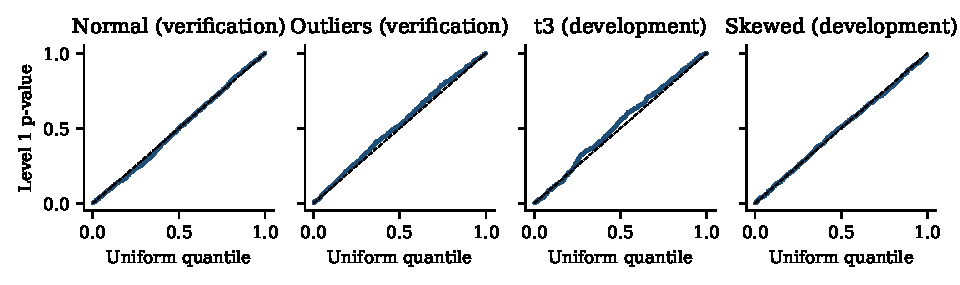
\includegraphics[width=\textwidth]{figures/fig_calibration.pdf}
\caption{Level 1 $p$-values under the null hypothesis against uniform quantiles, for four noise distributions (two verification and two development runs). The dashed line is the identity.}
\label{fig:calibration}
\end{figure}

\subsection{Across data sets, no $\Hone$ statistic separated the matched patterns}\label{sec:res-matched}
In the matched experiment, \nCentresOne{} of the \decOneN{} data sets at size 1 had one cycle centre, \nCentresTwo{} had two and \nCentresThree{} had three, with a median of \decOneChanged{} changed genes. Every directional statistic responded to the change, but by the pre-declared criterion no $\Hone$ statistic separated the cycle arm from the module arm: the AUC of $A_i$, its rank variant and $Z_i$ lay between 0.50 and \aucZTwo{} at both effect sizes (Table~\ref{tab:matched}). Signed Moran's $I$ (B2) separated the arms more strongly, in the opposite direction: its AUC was \aucBtwoOne{} and \aucBtwoTwo{}, an oriented AUC of \aucOrBtwoOne{} and \aucOrBtwoTwo{}, because in the module arm the centre changes together with its neighbours. Under the plan's rule, $\Hone$ therefore did not add information in this experiment. The variation between data sets, which differ in subnetwork and in the number of centres, was much larger than the difference between the arms.

The sign of $A_i$ is informative. A cycle of increased genes around an unchanged centre might be expected to raise $\Lup_i$ and make $A_i$ positive. Instead $A_i$ was strongly negative in both arms (mean $t=\tcycATwo$ in the cycle arm and $\tmodATwo$ in the module arm at size 2). We propose the following mechanism, which we have not verified at the level of individual intervals. In the lower-change filtration a block of increased genes enters last; the unchanged genes around it enter earlier and can form cycles that the block's genes fill when they enter, each with a lifetime close to the size of the change. Such cycles add to $\Ldown_i$ whether or not the block surrounds an unchanged gene, and they can be numerous. On an interaction network with many triangles, raw directional $\Hone$ persistence would then largely reflect where blocks of change sit, much like the $\Hzero$ asymmetry (B4, mean $t=\tcycBfourTwo$ and $\tmodBfourTwo$) and the component contrast (B3).

\begin{table}[t]
\centering\small
\caption{Matched cycle--module experiment, verification seeds (\decOneN{} data sets per size). Paired: share of data sets in which the statistic was larger in the cycle arm than in the module arm built from the same noise on the same subnetwork, with exact 95\% confidence intervals; there were \pairTies{} ties. $\Delta t$: mean paired difference $t_{\mathrm{cycle}}-t_{\mathrm{module}}$. AUC: $P(t_{\mathrm{cycle}}>t_{\mathrm{module}})$ over all pairs of data sets, ties counted one half; values below 0.5 mean the statistic is larger in the module arm. Size: change in units of the noise standard deviation.}
\label{tab:matched}
{\footnotesize\setlength{\tabcolsep}{4pt}\begin{tabular}{lrrrrrr}
\toprule
 & \multicolumn{3}{c}{Size 1} & \multicolumn{3}{c}{Size 2} \\
\cmidrule(lr){2-4}\cmidrule(lr){5-7}
Statistic & Paired (\%) & 95\% CI & AUC & Paired (\%) & 95\% CI & AUC \\
\midrule
$A_i$ (H1 asymmetry) & 61 & 54--68 & 0.51 & 72 & 65--78 & 0.52 \\
$A_i$, rank variant & 60 & 52--66 & 0.50 & 75 & 68--81 & 0.53 \\
$Z_i$ (network-adjusted) & 70 & 63--76 & 0.52 & 80 & 73--85 & 0.54 \\
B1 signed burden & 52 & 45--60 & 0.50 & 50 & 43--58 & 0.50 \\
B2 signed Moran's $I$ & 2 & 1--5 & 0.40 & 0 & 0--2 & 0.34 \\
B3 component size & 60 & 53--67 & 0.52 & 60 & 53--67 & 0.52 \\
B4 $H_0$ asymmetry & 44 & 37--51 & 0.47 & 44 & 37--51 & 0.47 \\
B9 local-extremum depth & 56 & 49--63 & 0.53 & 56 & 48--63 & 0.53 \\
\bottomrule
\end{tabular}
}
\end{table}

\subsection{Within matched pairs, the $\Hone$ statistics responded to the exchange}\label{sec:res-signal}
Holding the network and the noise fixed (Figure~\ref{fig:matched}), the $\Hone$ statistics were larger in the cycle arm than in its matched module arm more often than not, and more often at the larger effect size: $A_i$ in \pairAOne\% and \pairATwo\% of data sets at sizes 1 and 2, its rank variant in \pairArankOne\% and \pairArankTwo\%, and the network-adjusted $Z_i$ in \pairZOne\% (95\% CI \pairZOneci\%) and \pairZTwo\% (\pairZTwoci\%). At size 2 the mean paired difference of $Z_i$ was $\Delta t=\dtZTwo$ (95\% interval \dtciZTwo), and that of $A_i$ was \dtATwo. The topology-free statistics responded too, though less consistently: the local-extremum depth B9 was larger in the cycle arm in \pairBnineOne\% and \pairBnineTwo\% of data sets ($\Delta t=\dtBnineTwo$ at size 2), the component contrast B3 in \pairBthreeOne\% and \pairBthreeTwo\% ($\Delta t=\dtBthreeTwo$), and the $\Hzero$ asymmetry B4 in \pairBfourOne\% and \pairBfourTwo\% ($\Delta t=\dtBfourTwo$). The burden B1, which counts the same number of changed genes in both arms, behaved as a negative control (\pairBoneOne\% and \pairBoneTwo\%). Signed Moran's $I$ responded most strongly of all, in the opposite direction: B2 was larger in the cycle arm in only \pairBtwoOne\% and \pairBtwoTwo\% of data sets ($\Delta t=\dtBtwoTwo$ at size 2). The development runs, on different seeds, gave the same pattern ($Z_i$ in \devpairZOne\% and \devpairZTwo\%; Supplementary Table~\ref{tab:matcheddev}).

Paired wins and AUC are compatible. At size 2, $Z_i$ moved in the direction of the cycle arm in \pairZTwo\% of matched pairs, but by much less than its variation between networks, so it ordered data sets from different networks little better than chance. Because the exchange of centre and neighbour also changes the degrees, clustering and local autocorrelation of the changed genes, these paired results show that the $\Hone$ statistics are sensitive to this intervention; they do not show that the response is due to the hole, and they do not show that $\Hone$ carries information beyond the baselines jointly, which we have not tested.

\begin{figure}[t]
\centering
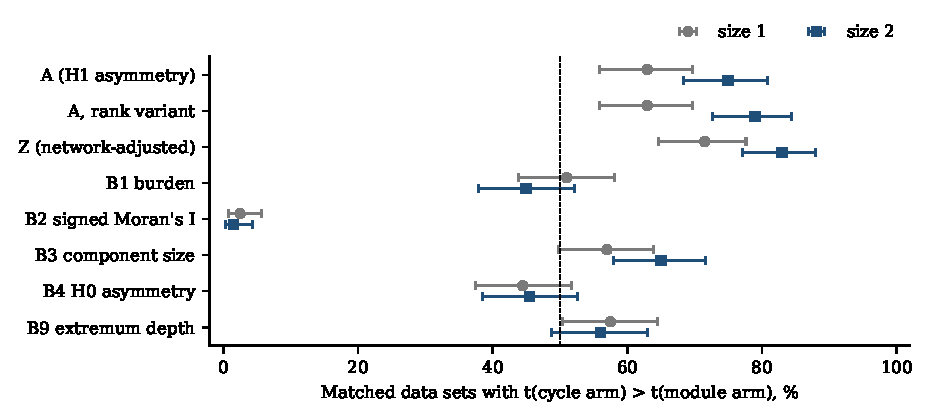
\includegraphics[width=\textwidth]{figures/fig_matched.pdf}
\caption{Matched cycle--module experiment. For each statistic, the share of matched data sets in which the statistic was larger in the cycle arm than in the module arm, with exact 95\% confidence intervals, at change sizes 1 (circles) and 2 (squares). There were no ties, so the dashed line at 50\% is the value expected if the exchange made no difference to the statistic.}
\label{fig:matched}
\end{figure}

\subsection{The network-adjusted reference did not absorb strong change at hubs}\label{sec:res-hub}
When only the genes in the top 5\% of degree changed, the raw asymmetry rejected $H_{\mathrm{sym}}$ in \hubA\% of \hubN{} data sets, as it should, since the change is real. The Level~2 test of $Z_i$ rejected in \hubZ\% of data sets (95\% CI \hubZci\%), and \hubZneg{} of the \hubZk{} rejections had a negative statistic. This is not a type~I error under $H_{\mathrm{sym}}$; it shows that the relabelling reference does not absorb this structured alternative, so that $Z_i$ would attribute it to arrangement. Two explanations are possible and we have not separated them. First, high-degree genes are interconnected in the graph used here: in the full STRING graph at score $\ge700$, the \hubHubN{} genes of the top 5\% of degree (degree $\ge\hubHubMinDeg$) share \hubHubObs{} edges, against a mean of \hubHubRew{} in \hubHubReps{} degree-preserving rewirings (ratio \hubHubRatio), and the degree assortativity is \degAssort. Relabelling within strata moves each hub's change to another gene of similar degree, but the genes that receive the changes are usually not adjacent, so the reference loses the adjacency among the changed hubs. This differs from the networks studied by \citet{maslov2002}, in which links between hubs were suppressed, and from the protein interaction network examined by \citet{colizza2006}, which showed no rich-club ordering; STRING includes members of protein complexes, which are densely linked. Second, the strata are coarse: the top 5\% of degree lies within the top decile, so relabelling within that decile moves changes to genes of lower degree even before adjacency is considered. A reference that preserves the adjacency among the changed genes would address the first explanation, and finer degree strata the second.

\subsection{Application to TCGA-BRCA}\label{sec:res-tcga}
The frozen analysis (Git tag \texttt{plan-v1.0}) was run on the \tcgaN{} patients. One technical amendment was made after the freeze and before any result was computed: arrays passed to GUDHI are copied, because GUDHI on Windows rejects the read-only memory-mapped arrays that the parallel back end uses for large inputs; it changes no value and is recorded in the file of amendments in \texttt{docs/provenance}. Table~\ref{tab:tcga} gives the patient-level results.

\paragraph{Paired asymmetry (Level 1).} The primary test rejected $H_{\mathrm{sym}}$ in both layers: RNA with $t=\tARna$ ($p_{\mathrm{Holm}}\pARna$; $A_i>0$ in \AposRna{} of \tcgaN{} patients) and methylation with $t=\tAMeth$ ($p_{\mathrm{Holm}}\pAMeth$; $A_i>0$ in only \AposMeth). The two results differ in robustness (Table~\ref{tab:tcgasens}). The RNA result changed sign with the rank variant ($t=\tArankRna$), the standardised change and both alternative network thresholds, and was not significant after composition adjustment or in pairs whose two specimens share a plate; it also weakened under added measurement noise (median $t$ \noiseTenRna, \noiseTwentyFiveRna{} and \noiseFiftyRna{} at 10\%, 25\% and 50\% of each gene's SD). The RNA Level~1 rejection is therefore not supported by the pre-specified sensitivity analyses. The methylation asymmetry was negative on the observed $M$-value scale in every pre-specified analysis except the rank variant ($t=\tArankMeth$), so it depends on the magnitudes of the changes and not only on their order; it was almost unchanged by noise (median $t$ \noiseFiftyMeth{} at 50\%). Its direction is the one that the proposed mechanism of Section~\ref{sec:res-matched} associates with connected blocks of increased change, and the non-topological baselines point the same way: more promoters were hypermethylated than hypomethylated among the analysed genes (B1, $t=\tBoneMeth$), and the hypermethylated genes formed larger components (B3, $t=\tBthreeMeth$) with stronger graph autocorrelation (B2, $t=\tBtwoMeth$). These statements concern the \methGenes{} analysed promoter-associated genes, not genome-wide methylation. Moran's $I$ of the change was positive on average in both layers. The two layers' asymmetries were weakly negatively correlated across patients (Spearman $\rho=\crossRho$, 95\% CI \crossRhoCI; exploratory).

\begin{table}[t]
\centering\small
\caption{TCGA-BRCA, \tcgaN{} tumour--normal pairs: studentized mean $t$ over patients and sign-flip $p$-value with Holm over the two layers ($B=9{,}999$, so the smallest attainable $p$ is $10^{-4}$). Upper block: topological statistics; the composition-adjusted $Z_i$ is an exploratory analysis decided after the frozen results were seen. Lower block: baselines on the same patients and sign flips.}
\label{tab:tcga}
\begin{tabular}{lrrrr}
\toprule
 & \multicolumn{2}{c}{RNA} & \multicolumn{2}{c}{Methylation} \\
\cmidrule(lr){2-3}\cmidrule(lr){4-5}
Statistic & $t$ & $p_{\mathrm{Holm}}$ & $t$ & $p_{\mathrm{Holm}}$ \\
\midrule
$A_i$ ($H_1$ asymmetry), Level 1 & +2.16 & 0.032 & -9.74 & $<$0.001 \\
$A_i$, rank variant & -2.37 & 0.038 & +1.19 & 0.231 \\
$Z_i$ (network-adjusted), Level 2 & +8.14 & $<$0.001 & +1.56 & 0.125 \\
$Z_i$, composition-adjusted (exploratory) & +6.38 & $<$0.001 & +1.97 & 0.057 \\
\midrule
B1 signed burden & +0.77 & 0.440 & +8.02 & $<$0.001 \\
B2 signed Moran's $I$ & -0.37 & 0.704 & +6.39 & $<$0.001 \\
B3 component size & +1.92 & 0.057 & +6.56 & $<$0.001 \\
B4 $H_0$ asymmetry & -15.20 & $<$0.001 & +10.27 & $<$0.001 \\
B9 local-extremum depth & +14.74 & $<$0.001 & -10.72 & $<$0.001 \\
B8 specimen-level $H_1$ & +6.83 & $<$0.001 & +5.92 & $<$0.001 \\
\bottomrule
\end{tabular}

\end{table}

\paragraph{Network-adjusted asymmetry (Level 2).} The reference used $R=199$ relabellings per patient within \methStrata{} (methylation) and \rnaStrata{} (RNA) non-empty strata; the reference spread fell below the floor in \atFloorRna{} (RNA) and \atFloorMeth{} (methylation) patients. For methylation the network-adjusted score was not significant ($t=\tZMeth$, $p_{\mathrm{Holm}}\pZMeth$; mean $Z_i=\ZmeanMeth$, 95\% CI \ZciMeth): the data do not show a systematic departure of the methylation asymmetry from the specified relabelling reference. This does not show that the arrangement of methylation changes is random on the network; B2 and B3 indicate that hypermethylated promoters are clustered. For RNA the network-adjusted score was consistent across patients but modest in each: $t=\tZRna$ ($p_{\mathrm{Holm}}\pZRna$), $Z_i>0$ in \ZposRna{} of \tcgaN, mean $Z_i=\ZmeanRna$ (95\% CI \ZciRna), median \ZmedRna, and $|Z_i|\le\ZmaxRna$ in every patient (Figure~\ref{fig:tcgaz}). The large $t$ reflects the consistency of a small departure across patients, not a large departure in any one. On the scale of the asymmetry, the observed $A_i$ averaged \AmeanRna{} against a reference mean of \AmuRna{} for the same changes relabelled within strata; the difference $A_i-\mu_i$ had median \AmuMedRna{} (interquartile range \AmuIQRRna). The raw RNA asymmetry was thus small and unstable, while its departure from the reference was consistent. Because composition was adjusted only at Level~1 in the plan, and composition removed the RNA Level~1 effect, we added one exploratory analysis after seeing these results: the same Level~2 test after regressing the stromal and immune proxies out of the change. The RNA score remained ($t=\tZcompRna$, $p_{\mathrm{Holm}}\pZcompRna$; $Z_i>0$ in \ZcompposRna{} patients); the mean $Z_i$ fell by \ZcompdropRna\%, and the adjusted and unadjusted scores were highly correlated across patients ($r=\ZcompcorrRna$). The methylation score stayed non-significant ($t=\tZcompMeth$). The simulations limit how the RNA result can be read: $Z_i$ is not specific to holes, and it responds to changed genes that are adjacent to one another (Section~\ref{sec:res-hub}). By the mechanism proposed in Section~\ref{sec:res-matched}, a positive $Z_i$ is consistent with connected groups of \emph{decreased} genes that fill cycles of the higher-change filtration, as well as with cycles of increased genes. Robustness analyses with a single relabelling applied to all patients, and with degree-preserving rewiring (which removed about 95\% of the triangles, \obsTriRna{} to a median of \rewireTriRna), showed that the Level~1 statistic depends strongly on the network's local structure (median $t$ \rewireTRna{} and \rewireTMeth{} on rewired networks; descriptive).

\begin{figure}[t]
\centering
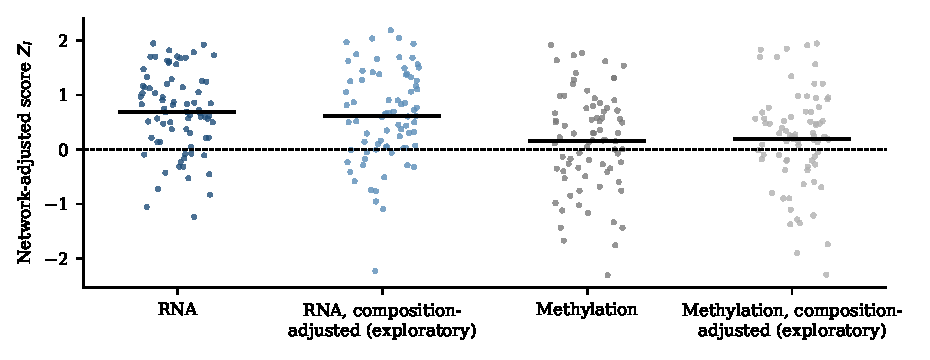
\includegraphics[width=\textwidth]{figures/fig_tcga_z.pdf}
\caption{Network-adjusted scores $Z_i$ of the \tcgaN{} patients, before and after the exploratory composition adjustment. Bars mark the means; the dashed line marks zero.}
\label{fig:tcgaz}
\end{figure}

\begin{table}[t]
\centering\small
\caption{Pre-specified sensitivity analyses of the Level~1 asymmetry $A_i$. The alternative STRING thresholds use the genes of the primary network (Section~\ref{sec:cohort}). Same-plate pairs: one layer each, unadjusted $p$.}
\label{tab:tcgasens}
\begin{tabular}{lrrrr}
\toprule
 & \multicolumn{2}{c}{RNA} & \multicolumn{2}{c}{Methylation} \\
\cmidrule(lr){2-3}\cmidrule(lr){4-5}
Analysis & $t$ & $p_{\mathrm{Holm}}$ & $t$ & $p_{\mathrm{Holm}}$ \\
\midrule
Primary (plain change, STRING $\ge$700) & +2.16 & 0.032 & -9.74 & $<$0.001 \\
Rank variant & -2.37 & 0.038 & +1.19 & 0.231 \\
Standardised change & -3.50 & 0.001 & -7.26 & $<$0.001 \\
STRING $\ge$400 & -6.50 & $<$0.001 & -13.95 & $<$0.001 \\
STRING $\ge$900 & -5.12 & $<$0.001 & -11.17 & $<$0.001 \\
Composition-adjusted & +1.56 & 0.119 & -8.77 & $<$0.001 \\
Same-plate pairs (60 / 45) & +1.45 & 0.157 & -9.22 & $<$0.001 \\
\bottomrule
\end{tabular}

\end{table}

\paragraph{Placebo.} In \placeboN{} data sets of pseudo-pairs formed from the tumours of different patients, Level~1 rejected in \placeboRna\% (RNA) and \placeboMeth\% (methylation) of data sets, in line with the nominal 5\% for this number of data sets.

\paragraph{Genes (Level 3).} Of the \geneFamily{} layer--gene pairs in the family (\audFamRna{} RNA, \audFamMeth{} methylation), \geneSig{} were significant after Holm (\geneSigRna{} RNA, \geneSigMeth{} methylation; smallest attainable $p=\minP$). These are layer--gene associations; they involve \geneUnique{} distinct genes. Each was stable by the pre-specified rule: in at least 50\% of 100 random half-samples of patients, its sign-flip test (999 flips) gave $p\le0.05$ with the same sign; all \geneStable{} met this rule. Under the reversed tie rule, \geneTiePct\% of the \geneSig{} kept the sign of their score; sign agreement does not show that representative membership is stable. The strongest RNA participants (Table~\ref{tab:tcgagenes}) are proliferation genes on cycles of the higher-change filtration (CCNA2, AURKA, PCNA, CDK1, CDC45, EZH2) together with FN1 and TGFB1, and vascular, stromal and adipose-associated genes on cycles of the lower-change filtration (VWF, ELN, DCN, CAV1, NID1, LRP1); the strongest methylation participants are dominated by immune genes. These match the known contrast between breast tumours and adjacent normal tissue \citep{tcga2012} and are consistent with differences in proliferation and in cell composition.

Table~\ref{tab:geneaudit} compares the topological participants with the single-gene test B6 and the smoothed test B7. As run, B6 and B7 used Holm over all genes of the layer network (\audNetRna{} RNA and \audNetMeth{} methylation), a larger family than the topology family; we also recomputed Holm for B6 over the topology family alone, which is the comparison on equal terms. On equal terms, \audNotBsixfRna{} of the \audTopoRna{} RNA participants (\audNotBsixfPctRna\%) and \audNotBsixfMeth{} of the \audTopoMeth{} methylation participants (\audNotBsixfPctMeth\%) were not significant as single genes; \audNotBothRna{} (\audNotBothPctRna\%) and \audNotBothMeth{} (\audNotBothPctMeth\%) were significant by neither B6 nor B7. A gene that is not significant after Holm can still have a substantial but variable change. In RNA, for example, DTNB was essentially unchanged (single-gene $t=\sgDtnb$), whereas SNTB1 ($t=\sgSntb$) and DAG1 ($t=\sgDag$) changed but did not reach Holm significance; all three belong to the dystrophin-associated protein complex. In methylation, the promoter of TNFRSF13C (the BAFF receptor) was unchanged as a single gene ($t=\sgBaffr$) but a strong participant, as was its ligand TNFSF13B ($t=\sgBaff$ as a single gene); we have not checked whether the two genes lie on the same cycle representatives, so their known interaction does not show co-attribution. Under the pre-declared outcome (below) these genes are candidates for follow-up, not gene-specific findings.

\begin{table}[t]
\centering\small
\caption{Topological participants compared with the single-gene test (B6) and the neighbourhood-smoothed test (B7), counted from the result files. Holm-significant at 0.05 throughout. ``Family Holm'': Holm recomputed over the topology family only, so that B6 and the topology test are adjusted over the same genes.}
\label{tab:geneaudit}
\begin{tabular}{lrr}
\toprule
 & RNA & Methylation \\
\midrule
Genes in the layer network (B6 and B7 were tested on all) & 7,624 & 8,438 \\
Topology family (non-zero score in $\ge$10 patients) & 2,595 & 2,823 \\
Topology: Holm-significant in its family & 833 & 446 \\
B6 single gene: Holm over network genes & 3,217 & 1,905 \\
B6 single gene: Holm over the topology family & 1,251 & 643 \\
B7 smoothed: Holm over network genes & 3,025 & 2,762 \\
\midrule
Topology, not B6 (Holm over network genes) & 333 & 221 \\
Topology, not B6 (Holm over the topology family) & 300 & 209 \\
Topology, not B7 & 460 & 182 \\
Topology, neither B6 nor B7 & 201 & 97 \\
\bottomrule
\end{tabular}

\end{table}

\begin{table}[t]
\centering\small
\caption{The 15 Holm-significant topological participants with the largest $|t|$ per layer. Positive $t$: on cycles of the higher-change filtration (increased genes); negative: of the lower-change filtration. Single-gene: Holm-significant in the paired single-gene test B6 (Holm over the network genes).}
\label{tab:tcgagenes}
\begin{tabular}{lrc|lrc}
\toprule
\multicolumn{3}{c|}{RNA} & \multicolumn{3}{c}{Methylation} \\
Gene & $t$ & Single-gene & Gene & $t$ & Single-gene \\
\midrule
FN1 & +22.9 & yes & CX3CL1 & +17.1 & yes \\
VWF & -21.5 & yes & CD40 & +14.7 & yes \\
CCNA2 & +20.4 & yes & TNFSF8 & -14.1 & yes \\
TGFB1 & +18.8 & yes & BICD2 & -14.0 & no \\
DTNB & +17.1 & no & RAB6A & -14.0 & no \\
PARP1 & +16.5 & yes & BICDL1 & -13.8 & no \\
ELN & -16.3 & no & TNFSF13B & -13.6 & no \\
PCNA & +16.1 & yes & CXCL1 & +13.2 & yes \\
SNTB1 & +16.1 & no & TNFRSF13C & -13.0 & no \\
AURKA & +15.9 & yes & PTEN & -12.8 & no \\
ATP6V0B & +15.7 & yes & CD80 & -12.3 & yes \\
CLSPN & +15.1 & yes & PSIP1 & -11.8 & no \\
RPA1 & -14.9 & no & ESR1 & -11.8 & yes \\
EGFR & -14.8 & yes & FGF2 & +11.4 & yes \\
TGFBR2 & -14.6 & yes & ITGB3 & +11.2 & yes \\
\bottomrule
\end{tabular}

\end{table}

\paragraph{Pre-declared outcome.} The plan defines the outcomes by whether Levels~1 and~2 are supported, without saying whether a primary rejection that the sensitivity analyses do not support counts as support. For methylation the answer does not matter: Level~1 rejected and kept its direction in every sensitivity analysis but the rank variant, and Level~2 did not reject, which is outcome C (directional asymmetry without demonstrated network specificity). For RNA it does. Reading ``supported'' as ``rejected in the primary test'', Levels~1 and~2 both rejected and the genes are unconfirmed, which is outcome B (a patient-level result without gene-specific claims). Reading it as ``rejected and robust'', Level~1 is not supported, which is outcome D for the paired asymmetry, with the Level~2 result reported as a secondary finding. We report both readings. Under either, the plan allows no gene-specific claims.

\section{Discussion}\label{sec:discussion}

We set out to make persistent homology of molecular change on an interaction network testable, and then to ask what it measures. Placing the signed paired change on a fixed complex and comparing the two directions of the lower-star filtration gives a statistic that reverses sign exactly when tumour and normal are exchanged (Proposition~\ref{prop:antisym}). That one property gives exact sign-flip tests with the patient as the unit of inference, and it carries over to a network-adjusted score (Proposition~\ref{prop:Z}), to a gene-level participation score and to every directional baseline. The tie rule is needed for this: it orders tied values by a fixed gene index without changing them, so that the two directions are exact mirror images even when measured changes are equal. In our simulations the Level~1 test and the gene family did not show excess rejection under four noise distributions, on development seeds and again on reserved verification seeds.

What the statistic measures is less favourable to a ring-based reading. A natural interpretation of a persistent $\Hone$ class on a network is a ring of changed genes around a gene that behaves differently. In our matched experiment, the pre-declared comparison across data sets favoured no $\Hone$ statistic, and signed Moran's $I$ separated the two arms better. Within matched pairs, the $\Hone$ statistics did respond to exchanging the centre with a neighbour: at the larger effect size the network-adjusted score rose in \pairZTwo\% of pairs. But the exchange also changed local autocorrelation, degree and clustering among the changed genes, and the topology-free statistics B3 and B9 moved in the same direction, by mean amounts similar to that of $A_i$. In both arms the raw asymmetry was strongly negative, which suggests that the lower-change filtration is dominated by cycles that a block of increased genes fills when it enters; we propose this mechanism but have not verified it interval by interval. In a noiseless planted subgraph the two arms differ cleanly, since the module arm's changed set induces a cone with no $\Hone$; on the full noisy network that difference is diluted by many other classes, and we did not measure how much of it survives.

The behaviour of the network-adjusted score under hub change is the second lesson. Relabelling a patient's changes within strata of degree and clustering is a common way to ask whether an arrangement is more than expected from the nodes involved. On the STRING graph, in which the highest-degree genes share \hubHubRatio{} times as many edges as degree-preserving rewiring predicts, the reference did not absorb strong change at those genes. A reference must preserve what the alternative is meant to exclude, here the adjacency among the changed genes, or the test will attribute that adjacency to arrangement; finer degree strata would also be needed. Degree-preserving rewiring of the whole graph is not such a reference, because it does not preserve the subgraph induced by the changed genes and, on this network, removes most triangles.

These findings bear on applications of persistent homology to functions on molecular and other networks \citep{masoomy2021,ramos2025,song2023,abdullahi2025,lee2012}. They do not show that such analyses are wrong. They show that a persistent loop, or a difference in total persistence, should be compared with simpler network statistics before it is interpreted as ring-like structure. The framework here supplies the tools for that comparison: a paired design with an exact test, a matched benchmark, and baselines computed on the same data with the same sign flips. We suggest that studies report, alongside any $\Hone$ finding, the corresponding $\Hzero$, component-size and Moran's $I$ results, and a null model that preserves the adjacency of the genes involved.

Three analyses would sharpen these conclusions. First, the matched experiment should record, for every data set, whether the planted class survives in the full filtration and what lifetime it contributes, so that the part of the paired response due to the planted class can be separated from the rest. Second, whether $\Hone$ adds information beyond the baselines jointly can be tested directly, by comparing a classifier of the two arms built from Moran's $I$, component size and burden with the same classifier after adding $\Hone$, on held-out data sets with both arms of each data set in the same split. Third, extended persistence \citep{cohensteiner2009}, which treats both directions of a function in one diagram and separates classes by type, may isolate hole-like classes more cleanly. Each should be one pre-declared endpoint evaluated on new simulation seeds and reported whatever the outcome; adding several constructions after seeing these results would trade the calibration that is the framework's main strength for a higher chance of a positive finding.

Persistent homology has properties that the baselines lack: it summarises every threshold at once, so its answer does not depend on a cut-off such as the $\tau$ of B1 and B3, and its cycle representatives say where on the network a signal lies. Whether these properties translate into better detection when change sizes differ from patient to patient has not been tested here.

The breast cancer analysis illustrates both lessons. The methylation asymmetry was the strongest topological result. It kept its direction under standardisation, both alternative network thresholds, composition adjustment and the same-plate restriction, but not under rank transformation, and simple counts, component sizes and autocorrelation pointed the same way. A reader who saw only the persistence diagrams might have described it as rings of hypomethylated genes; the baselines are more simply described as more, and more clustered, hypermethylation of the analysed promoters in tumours. The network-adjusted score did not show a departure from the relabelling reference. The RNA result is the reverse case. The raw asymmetry was fragile and changed sign between reasonable analysis choices, while the network-adjusted score was positive in most patients, modest in each, and remained after an exploratory composition adjustment. We read it as evidence that tumour--normal RNA changes are arranged on the interaction network differently from the same changes placed at random positions of similar degree, clustering and expression. We do not read it as evidence of rings: the score is not specific to holes, and connected groups of co-decreased genes, such as vascular, stromal and adipose programmes, would produce it. The composition proxies cover stroma and immune cells but not adipocytes, which are abundant in normal breast, and an independent cohort is needed before the result can be called confirmed. At the gene level, about a third of the RNA participants and about half of the methylation participants were not significant as single genes on equal terms, and about a quarter and a fifth were also missed by neighbourhood smoothing. Such genes are candidates for follow-up because their network neighbourhood changes; whether they matter in their own right is not something these data can show.

\section{Limitations}\label{sec:limitations}

\paragraph{Simulation.} The simulation study uses subnetworks of 400 and 800 genes, a single network score threshold and a simple patient model with a shared component and independent errors. The shared component cancels from the plain change, and the difference of two independent gamma errors is symmetric, so the model does not test correlated changes along pathways, heterogeneous changes between patients or tissue composition. The Level~2 test was not run under a complete null with the final reference. The matched experiment plants one to three centres of a single kind and two effect sizes; it exchanges a centre with a neighbour, which changes more than the presence of a hole; and it does not record whether the planted class survives in the full filtration. Whether $\Hone$ adds information to the baselines jointly was not tested. The network-adjusted score used $R=19$ relabellings per patient in the simulations, fewer than the 199 used for the real data, and its simulated reference was stratified by degree and clustering only. The null calibration with normal and outlier noise and the matched experiment were repeated on reserved verification seeds with the final code; the heavy-tailed and skewed null runs and the hub-change run were made on development seeds only.

\paragraph{Inference.} Validity of the tests is validity under $H_{\mathrm{sym}}$, the exchangeability of each patient's two specimens. In real data this can fail for technical reasons, such as tumour and normal specimens processed on different plates, and adjacent normal tissue is not healthy tissue: it can carry field effects, and both specimens are mixtures of cell types. A rejection therefore shows a paired difference in directional topology, not its cause. For the gene family, family-wise error control is established under the complete null; under a partial null, the validity of each unaffected gene's $p$-value conditionally on a family selected from all genes has not been shown (Section~\ref{sec:inference}). Cycle representatives are deterministic but not canonical; gene scores depend on them, and we checked only the sign of each score under one alternative tie rule.

\paragraph{Network and data.} STRING edges include indirect associations such as shared complex membership, and filling 3-cliques is a modelling choice; cycles describe arrangements of assay values on a reference graph. The methylation value of a gene is a median of promoter-probe $M$-values, and statements about hypermethylation concern the analysed promoter-associated genes, not genome-wide methylation. The composition adjustment uses RNA-derived stromal and immune proxies only, applies them to the methylation layer as well, and is exploratory at Level~2. The alternative network thresholds (STRING scores 400 and 900) were applied to the genes of the primary network rather than to each network's own gene set, because the preprocessed data hold only those genes.

\paragraph{Cohort.} The TCGA-BRCA cohort has \cohortN{} eligible pairs, a single source and a cross-sectional design. Independent confirmation is planned in the Hong Kong breast cancer cohort (dbGaP phs001870, controlled access; paired tumour and adjacent normal tissue with RNA sequencing and EPIC methylation profiling), with network, gene universe, preprocessing and code frozen before those data are opened; the number of patients with both layers in both tissues will be reported once access is granted. A data access request has been drafted.


\section*{Code, data and reproducibility}
All code, the analysis plan, the simulation result files and the data provenance records are in the public repository \coderepo{} (Python; \todo{add a licence file, e.g.\ MIT, before submission}). Every result file used in this version is in the repository at commit \resultscommit{}; Table~\ref{tab:provenance} lists each file with its SHA-256 hash, and the script \texttt{scripts/paper\_numbers.py} computes every number, table and figure of this paper from those files and writes them to this manuscript's \texttt{generated/} and \texttt{figures/} folders, so that no reported number is typed by hand. Simulations are run with \texttt{scripts/sim\_suite.py}; each run is resumable and uses its own pre-assigned seed range (development seeds from 1, verification seeds from 100{,}000); the verification runs were made once, on the final code. The unit tests (\texttt{python -m pytest}) check, among other things, every cycle representative against an independent boundary-matrix reduction and the exact sign reversal of every directional statistic. The analysis plan (\texttt{docs/analysis\_plan.md}) will be frozen by the Git tag \texttt{plan-v1.0} before any tumour-versus-normal outcome of patient data is computed; every access to patient molecular values is logged in \texttt{docs/provenance/access\_ledger.md}. The manuscript source is maintained in a separate repository synchronised with Overleaf. \todo{archive the tagged release on Zenodo and cite its DOI.}

TCGA-BRCA data are open-access files of the NCI Genomic Data Commons; the file manifest with hashes is in \texttt{docs/provenance}. The two STRING v12.0 files used (human physical links and protein information) are recorded with their SHA-256 hashes in the same folder.

\begin{table}[H]
\centering\footnotesize
\caption{Simulation result files used in this paper (repository \coderepo, commit \resultscommit). Hashes are of the files with LF line endings, the form stored in Git.}
\label{tab:provenance}
\begin{tabular}{lllrl}
\toprule
Seeds & Result file & Run & Data sets & SHA-256 (first 16) \\
\midrule
verification & \texttt{level1\_null\_normal.csv} & Null, normal & 1,000 & \texttt{078e616e384148b1} \\
verification & \texttt{level1\_null\_outliers.csv} & Null, outliers & 500 & \texttt{a1d8e8c7e34ff3ea} \\
verification & \texttt{decisive\_s1.csv} & Matched, size 1 & 200 & \texttt{cfc93cedd07482b3} \\
verification & \texttt{decisive\_s2.csv} & Matched, size 2 & 200 & \texttt{675377bf2b6bf311} \\
development & \texttt{level1\_null\_normal\_std.csv} & Null, normal & 1,000 & \texttt{d6ced790a2f5a8be} \\
development & \texttt{level1\_null\_t3\_std.csv} & Null, $t_3$ & 500 & \texttt{e4c7801f11886cbd} \\
development & \texttt{level1\_null\_skewed\_std.csv} & Null, skewed & 500 & \texttt{c6902d8d2e37b8a0} \\
development & \texttt{decisive\_s1.csv} & Matched, size 1 & 200 & \texttt{bb719979c9c548e1} \\
development & \texttt{decisive\_s2.csv} & Matched, size 2 & 200 & \texttt{f7a69c575b5b29ba} \\
development & \texttt{net\_hub\_de.csv} & Hub change (N3) & 500 & \texttt{151dbf7f74c41f16} \\
\bottomrule
\end{tabular}

\end{table}

\section*{Acknowledgements}
This work was supported by ICSR Grant No.\ RF24250543MARFER008771, IIT Madras. We thank The Cancer Genome Atlas and the patients who contributed specimens.
\todo{Author contributions and further acknowledgements: to be added by the authors.}

\bibliographystyle{plainnat}
\bibliography{references}

\clearpage
\appendix
\renewcommand{\thesection}{S\arabic{section}}
\section*{Supplementary material}
\section{Analysis plan}\label{sec:plan}

The complete analysis plan is \texttt{docs/analysis\_plan.md} in the code repository \coderepo. It was written before any tumour-versus-normal outcome of patient data was computed and frozen by the Git tag \texttt{plan-v1.0} (commit \texttt{8443cee}), whose SHA-256 is recorded in \texttt{docs/provenance}. Its main elements are listed here.

\paragraph{Hypotheses, in order.} $H_{\mathrm{sym}}$: within each patient tumour and normal profiles are exchangeable (Level 1, sign-flip test of $A_i$). $H_{\mathrm{net}}$: the network-adjusted asymmetry $Z_i$ is sign-symmetric (Level 2). $H_{\mathrm{gene}}(g)$: the gene score $a_i(g)$ is sign-symmetric (Level 3, Holm over the whole gene family). Rejecting one does not imply rejecting another.

\paragraph{Pre-declared outcomes.} (A) Levels 1 and 2 supported, genes stable and confirmed in the independent cohort: reproducible, network-specific directional organisation with replicated signature genes. (B) Levels 1 and 2 supported, genes unstable or unconfirmed: a patient-level result without gene-specific claims. (C) Level 1 supported, Level 2 not: directional asymmetry without demonstrated network specificity. (D) Level 1 not supported: a calibrated negative result. In every outcome the comparison with baselines B1--B9 is reported. The plan does not define ``supported'' further; Section~\ref{sec:res-tcga} reports both readings for RNA.

\paragraph{Matched experiment.} The plan states: ``If $A_i$ or $Z_i$ separates the arms better than B2, B3, B4 and B9, $\Hone$ adds information here. If a simpler statistic does as well, the paper says so.'' Separation was to be summarised by the AUC across data sets.

\paragraph{Claims not made.} That a cycle or module is a pathway or mechanism; that a gene causes the difference; that the data show how a tumour develops; that topology finds information absent from the molecular data (the diagrams are functions of the change and the network); that a new topological construction is introduced; that a replicated signature gene is a clinical biomarker; that a result attenuated by composition adjustment reflects regulation within tumour cells.

\paragraph{Simulation gates.} Each null run passes if the one-sided exact binomial test of ``rejection rate $\le0.05$'' gives $p\ge0.01$. Development and verification seed ranges are separate; the verification runs are made once on the final code, and their results are the ones reported in the main text. Table~\ref{tab:matcheddev} gives the matched experiment on development seeds.

\begin{table}[H]
\centering\small
\caption{Matched cycle--module experiment on development seeds (\devdecOneN{} data sets per size); columns as in Table~\ref{tab:matched}.}
\label{tab:matcheddev}
{\footnotesize\setlength{\tabcolsep}{4pt}\begin{tabular}{lrrrrrrrr}
\toprule
 & \multicolumn{4}{c}{Size 1} & \multicolumn{4}{c}{Size 2} \\
\cmidrule(lr){2-5}\cmidrule(lr){6-9}
Statistic & Paired (\%) & 95\% CI & $\Delta t$ & AUC & Paired (\%) & 95\% CI & $\Delta t$ & AUC \\
\midrule
$A_i$ (H1 asymmetry) & 61 & 54--68 & +0.09 & 0.51 & 72 & 65--78 & +0.48 & 0.52 \\
$A_i$, rank variant & 60 & 52--66 & +0.10 & 0.50 & 75 & 68--81 & +0.67 & 0.53 \\
$Z_i$ (network-adjusted) & 70 & 63--76 & +0.25 & 0.52 & 80 & 73--85 & +0.80 & 0.54 \\
B1 signed burden & 52 & 45--60 & -0.00 & 0.50 & 50 & 43--58 & -0.00 & 0.50 \\
B2 signed Moran's $I$ & 2 & 1--5 & -0.56 & 0.40 & 0 & 0--2 & -2.44 & 0.34 \\
B3 component size & 60 & 53--67 & +0.14 & 0.52 & 60 & 53--67 & +0.23 & 0.52 \\
B4 $H_0$ asymmetry & 44 & 37--51 & -0.25 & 0.47 & 44 & 37--51 & -0.50 & 0.47 \\
B9 local-extremum depth & 56 & 49--63 & +0.24 & 0.53 & 56 & 48--63 & +0.51 & 0.53 \\
\bottomrule
\end{tabular}
}
\end{table}

\paragraph{Pre-specified and exploratory analyses.} Table~\ref{tab:prespec} lists every analysis of the TCGA data by endpoint.

\begin{table}[H]
\centering\footnotesize
\caption{Analyses of the TCGA-BRCA data. Pre-specified: in the frozen plan (tag \texttt{plan-v1.0}). Exploratory: decided after the frozen results were seen.}
\label{tab:prespec}
\begin{tabular}{p{0.2\textwidth}p{0.46\textwidth}p{0.26\textwidth}}
\toprule
Endpoint & Analysis & Status \\
\midrule
Level 1, $A_i$ & Primary test, both layers, Holm over layers & Pre-specified \\
Level 1, $A_i$ & Rank variant; standardised change; STRING $\ge$400 and $\ge$900; composition adjustment; same-plate pairs & Pre-specified (sensitivity) \\
Level 1, $A_i$ & Added measurement noise; one relabelling for all patients; degree-preserving rewiring & Pre-specified (descriptive) \\
Level 1, $A_i$ & Placebo pseudo-pairs of tumours & Pre-specified (pipeline check) \\
Level 2, $Z_i$ & Primary test, both layers, Holm over layers & Pre-specified \\
Level 2, $Z_i$ & Composition adjustment & Exploratory \\
Level 3, genes & Holm over the family; half-sample stability; reversed tie rule & Pre-specified \\
Level 3, genes & B6 with Holm over the topology family; overlap with B7 & Exploratory \\
Baselines & B1--B4, B8, B9 on the same sign flips; B6, B7 & Pre-specified \\
Cross-layer & Spearman correlation of $A_i$ between layers & Pre-specified, exploratory \\
Network & Hub--hub edges against degree-preserving rewiring (no patient data) & Exploratory \\
\bottomrule
\end{tabular}
\end{table}

\paragraph{Changes made after results were seen.} The matched experiment, the network-adjusted score and baseline B9 were added to the plan before their simulations were run. No endpoint has been added or changed after its simulation results were seen. After the freeze, one technical amendment (copies of arrays passed to GUDHI; no effect on any value) was made before results were computed. The analyses marked exploratory in Table~\ref{tab:prespec} were added after the frozen results were seen; all are recorded in the repository. The STRING 400 and 900 sensitivity analyses used the genes of the primary network.


\end{document}
